\section{Bootstrapowane DQN - prosta implementacja}
Celem tego eksperymentu było zaimplementowanie prostej wersji Bootstrapowanej DQN opisanej w \cite{DBLP:journals/corr/OsbandBPR16} i sprawdzenie jej zachowania pod względem kierowania eksploracją i modelowania niepewności agenta.

\subsection{Implementacja}
Zaproponowana w \cite{DBLP:journals/corr/OsbandBPR16} wersja ostateczna BDQN opiera się na jednej głębokiej sieci neuronowej, w której najwyższe warstwy ,,rozdzielały się'' na $K$ różnych ,,głów'' sieci, gdzie każda głowa odpowiadała jednej funkcji Q. Każda z funkcji Q jest uczona na podstawie osobnego próbkowanego zestawu danych, do którego z zadanym prawdopodobieństwem $p$ dołączane są wygenerowane podczas uczenia próbki. Na początku każdego epizodu losowo wybierana jest aktywna głowa, która w danym epizodzie będzie służyła za funkcję Q - dzięki temu zachowanie agenta w ramach każdego epizodu jest nieco różne, ale spójne.

Uproszczona wersja BDQN wspomniana w artykule i zaimplementowana w tym eksperymencie zakłada wykorzystanie $K$ niezależnych sieci zamiast jednej sieci z wieloma ,,głowami''. Warto zwrócić uwagę, że to uproszczona implementacja dokładniej realizuje bootstraping, zapewniając niezależność sieci - w łączonej sieci górne warstwy uczyły się na próbkowanych danych, natomiast dolne uczyły się na pełnym zbiorze - kosztem niezależności znacznie skrócono czas uczenia.

Miarę pewności sieci, mierzoną dla każdej podjętej decyzji, przyjęto jako liczbę głów zgadzających się z decyzją aktywnej głowy podzieloną przez liczbę głów $K$. Ostateczna miara pewności dla danego epizodu była uśrednioną wartością pewności wszystkich decyzji podjętych w tym epizodzie.

\subsection{Ustawienia}
Eksperyment przeprowadzono przy użyciu scenariusza \textit{basic}. Punktem odniesienia był przykładowy agent dostarczony przez autorów VizDooma, opierający się na DQN. Kod agenta (a w szczególności architektura sieci neuronowej) posłużyła za podstawę eksperymentalnego agenta wykorzystującego BDQN. Dzięki temu jedynym zmiennym elementem w eksperymencie było badane bootstrapowanie danych dla sieci.

Eksperymenty przeprowadzano dla liczby podsieci $K=5,10$ i prawdopodobieństwa uwzględnienia próbki $p=0.5,0.75,0.9,1$. Agenci uczyli się przez $20$ epok po $2000$ epizodów każda. Celem eksperymentu było wstępne zbadanie przydatności BDQN i zaobserwowanie ogólnych trendów, dlatego badania nie były wielokrotnie powtarzane.

\subsection{Wyniki}
Eksperyment wykazał, że BDQN może uczyć się znacznie szybciej (w kontekście liczby epizodów, nie czasu) niż zwykła DQN. Dodatkowo przyjęta miara pewności sieci wyraźnie koreluje z wynikami uzyskiwanymi przez agenta.

Jak widać na wykresie \ref{fig:naive_bdqn_test_scores}, wyniki BDQN przekraczają granicę 0 i dochodzą do ostatecznych wartości kilka epok wcześniej niż DQN. Wszystkie rozwiązania zbiegają się do porównywalnych wyników - empiryczna analiza zachowań agenta wskazuje, że nie jest to jeszcze zachowanie optymalne, ale sensowne. Akcje agenta sugerują niedokładność percepcji, co może wskazywać na zbyt prostą lub zbyt małą sieć.
Zaimplementowane BDQN działa szybciej biorąc pod uwagę epoki, ale nie czas. Prostota implementacji sprawia, że odbycie każdej epoki zajmuje BDQN do trzech razy więcej czasu niż DQN. Spodziewane jest, że docelowa implementacja będzie porównywalna z DQN.

Ciekawe jest zachowanie BDQN dla różnych zestawów parametrów. Autorzy \cite{DBLP:journals/corr/OsbandBPR16} osiągali najlepsze wyniki dla $p=0.5$ i rosnące nieznacznie wraz ze wzrostem $K$. Badany agent dla $p=0.5$ osiągał gorsze wyniki niż DQN. Jest to zrozumiałe zachowanie - w docelowej implementacji część sieci uczona jest w praktyce na wszystkich danych, podczas gdy badane rozdzielne sieci dla $p=0.5$ są w każdym momencie nauczone dwa razy mniejszym zestawie danych niż analogiczny agent DQN. Warto zwrócić uwagę, że dzięki losowej inicjalizacji wag nawet dla $p=1$ uzyskane podsieci nie są identyczne.

Wyniki gorsze dla $K=10$ niż dla $K=5$ są natomiast sprzeczne z oczekiwaniami, przy czym to zachowanie nie wydaje się istotne przy badaniu na najprostszym scenariuszu.

\begin{figure}[H]
    \centering
    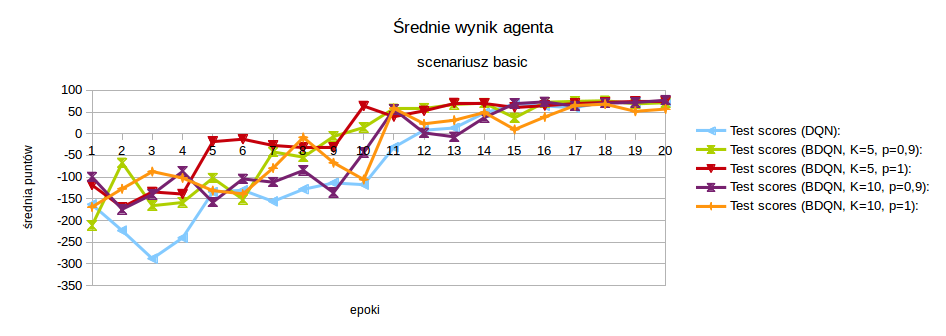
\includegraphics[width=0.95\textwidth]{figures/figures/naive_bdqn_test_scores.png}
    \caption{Średnie wyniki agentów dla scenariusza \textit{basic}}
    \label{fig:naive_bdqn_test_scores}
\end{figure}

Jak widać na wykresie \ref{fig:naive_bdqn_certainties}, pewność estymatora wyraźnie rośnie w miarę uczenia i koreluje z wynikami uzyskiwanymi przez agentów.

\begin{figure}[H]
    \centering
    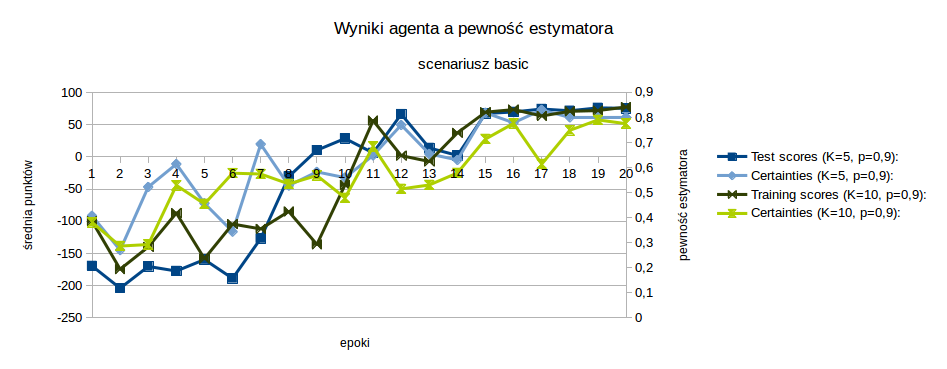
\includegraphics[width=0.95\textwidth]{figures/figures/naive_bdqn_certainties.png}
    \caption{Średnie wyniki a pewność estymatora dla scenariusza \textit{basic}}
    \label{fig:naive_bdqn_certainties}
\end{figure}

\subsection{Wnioski}
Eksperyment z użyciem prostej implementacji BDQN i prostego scenariusza \textit{basic} wykazał, że BDQN ma potencjał prowadzenia skutecznej eksploracji samo w sobie, a co ważniejsze, umożliwia sensowne estymowanie stopnia pewności sieci, co stanowi podstawę do bardziej zaawansowanych technik kierowania eksploracją.
